\chapter{Конструкторский раздел}

\section{Последовательность действий ПО}

На рисунке~\ref{fig:idef00} представлена диаграмма IDEF0, описывающая последовательность действий ПО.

\begin{figure}[H]
	\centering
	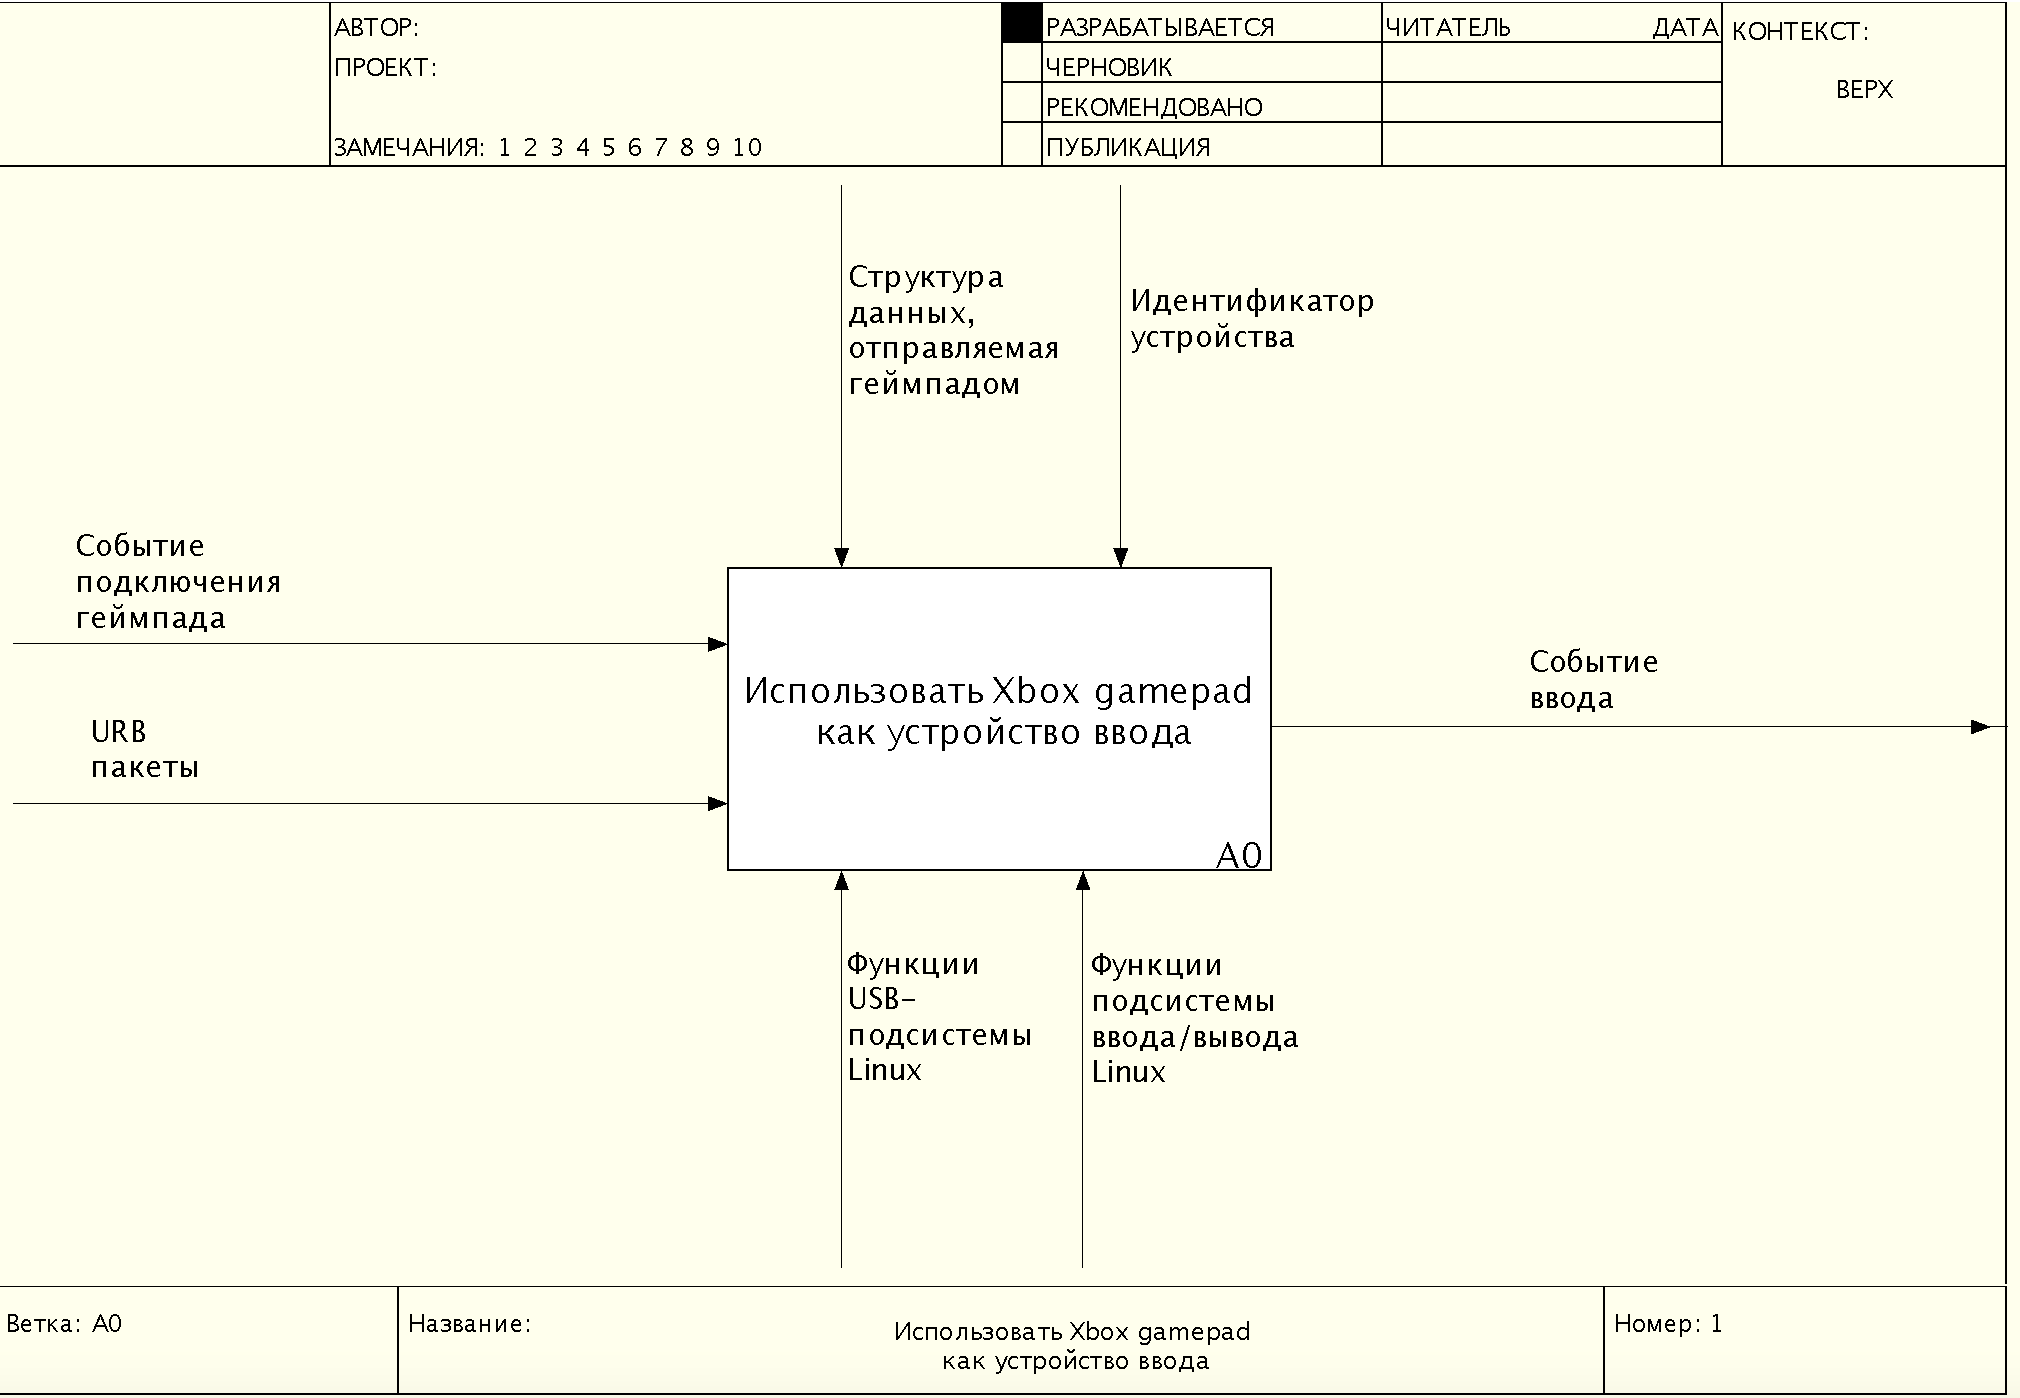
\includegraphics[width=0.8\textwidth]{images/01_A0.png}
	\caption{Диаграмма IDEF0 нулевого уровня}
	\label{fig:idef00}
\end{figure}

\section{Архитектура драйвера}

Драйвер Xbox Series S имеет модульную архитектуру, состоящую из следующих основных компонентов:
\begin{itemize}[label=---]
    \item Модуль инициализации и регистрации USB-драйвера;
    \item Обработчик входящих пакетов данных от контроллера;
    \item Подсистема эмуляции мыши;
    \item Механизм отправки команд контроллеру.
\end{itemize}

На рисунке~\ref{fig:po_struct} представлена общая структура ПО.

\begin{figure}[H]
	\centering
	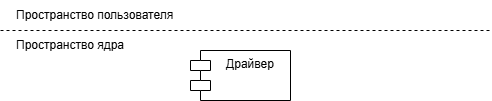
\includegraphics[width=0.8\textwidth]{images/po_struct.png}
	\caption{Структура ПО}
	\label{fig:po_struct}
\end{figure}

\section{Алгоритм обработки ввода}

На рисунке \ref{fig:handler} представлена схема алгоритма обработки входящих данных от контроллера.

\begin{figure}[H]
	\centering
	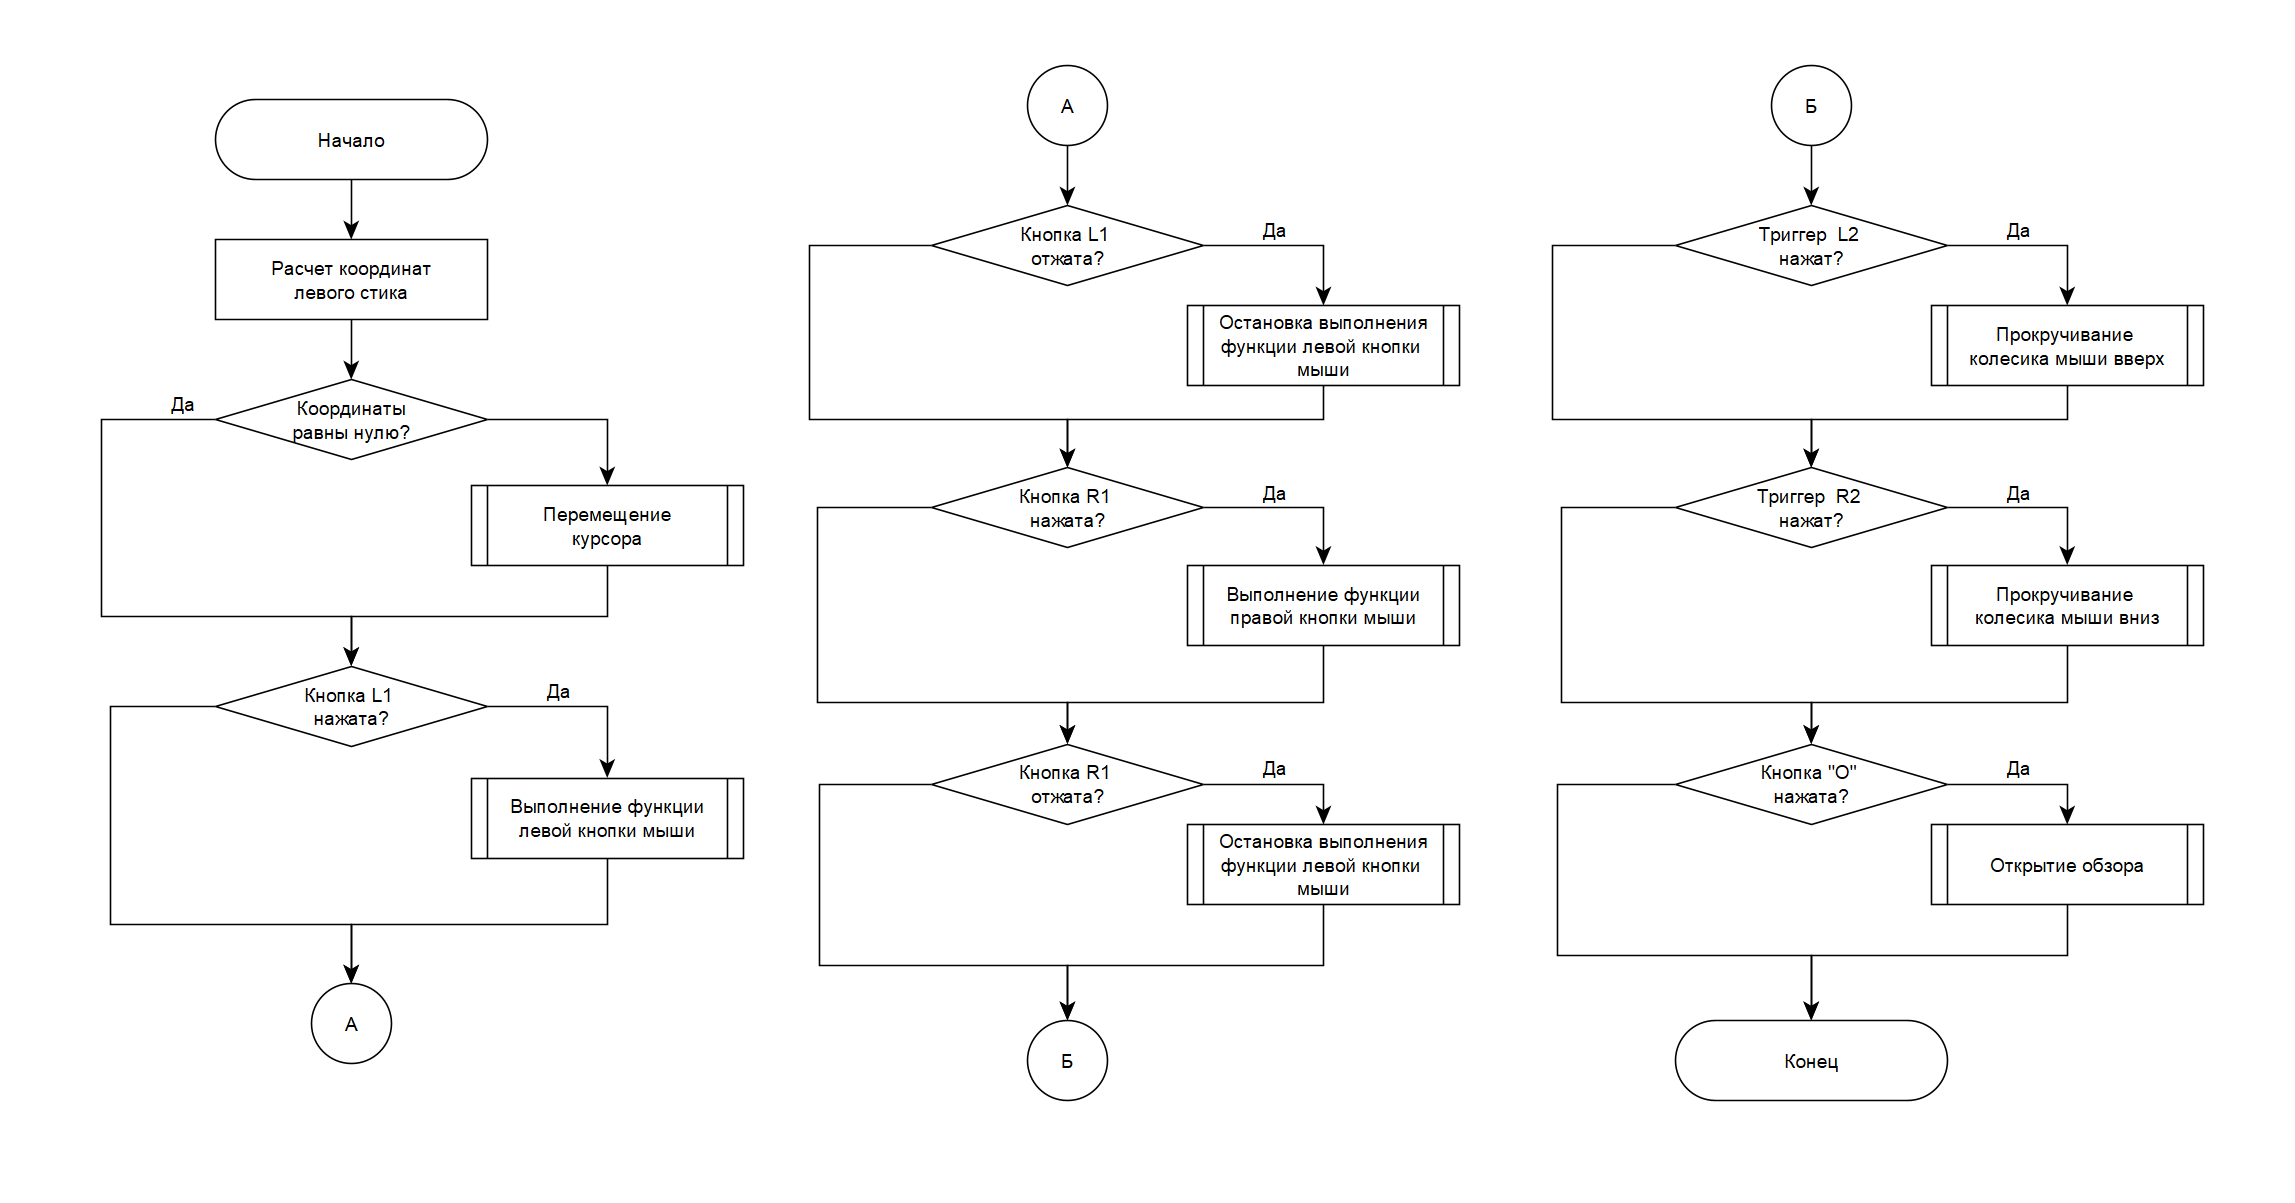
\includegraphics[width=1\textwidth]{images/iohandler.png}
	\caption{Схема алгоритма обработки ввода}
	\label{fig:handler}
\end{figure}

\section{Алгоритм эмуляции мыши}

Эмуляция мыши реализована через преобразование данных от аналоговых стиков:
\begin{itemize}[label=---]
    \item Левый стик (ось X) преобразуется в относительное горизонтальное перемещение курсора мыши;
    \item Правый стик (ось Y) преобразуется в относительное вертикальное перемещение курсора мыши;
    \item Кнопки контроллера эмулируют кнопки мыши: A → левая, B → правая, X - средняя.
\end{itemize}

Для обработки перемещения курсора применяется алгоритм с мертвой зоной и регулируемой чувствительностью. На рисунке \ref{fig:cur_alg} представлена схема алгоритма перемещения курсора.

\begin{figure}[H]
	\centering
	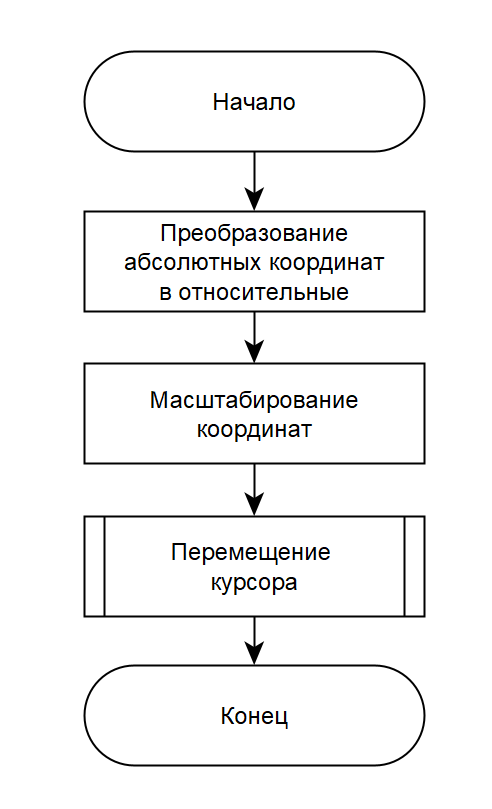
\includegraphics[width=0.35\textwidth]{images/cursor_alg.png}
	\caption{Схема алгоритма перемещения курсора}
	\label{fig:cur_alg}
\end{figure}

Параметры настройки:
\begin{itemize}[label=---]
    \item \texttt{mouse\_sensitivity} — чувствительность движения курсора (1-10);
    \item \texttt{scroll\_sensitivity} — чувствительность прокрутки (1-10);
    \item \texttt{mouse\_deadzone} — мертвая зона для исключения случайных движений.
\end{itemize}

\section{Инициализация контроллера}

Для корректной работы Xbox Series S контроллера требуется специальная последовательность инициализации:
\begin{enumerate}
    \item Отправка пакета питания \texttt{xboxone\_power\_on};
    \item Ожидание подтверждения от контроллера;
    \item Настройка конечных точек USB для приема и передачи данных;
    \item Регистрация устройств ввода в системе.
\end{enumerate}